\documentclass[12pt,a4paper]{report}
\usepackage{todonotes}

\usepackage[utf8]{inputenc} % pentru suport diacritice
\usepackage[romanian]{babel} % setări pentru limba română 
\renewcommand\familydefault{\sfdefault} % sans serif

\usepackage[margin=2.54cm]{geometry}	% dimensiuni pagină și margini
\usepackage{graphicx} % support the \includegraphics command and options

% formatting sections and subsections
\usepackage{textcase}
\usepackage[titletoc, title]{appendix}
\usepackage{titlesec}
\titleformat{\chapter}{\large\bfseries}{\thechapter}{2ex}{}[\vspace*{-1.5cm}]
\titleformat*{\section}{\large\bfseries}
\titleformat*{\subsection}{\large\bfseries}
\titleformat*{\subsubsection}{\large\bfseries}

\usepackage{chngcntr}
\counterwithout{figure}{chapter} % no chapter number in figure labels
\counterwithout{table}{chapter} % no chapter number in table labels
\counterwithout{equation}{chapter} % no chapter number in equation labels

\usepackage{booktabs} % for much better looking tables
\usepackage{url} % Useful for inserting web links nicely
\usepackage[bookmarks,unicode,hidelinks]{hyperref}

\usepackage{array} % for better arrays (eg matrices) in maths
\usepackage{paralist} % very flexible & customisable lists (eg. enumerate/itemize, etc.)
\usepackage{verbatim} % adds environment for commenting out blocks of text & for better verbatim
\usepackage{subfig} % make it possible to include more than one captioned figure/table in a single float
\usepackage{enumitem}
\setlist{noitemsep}

%%% HEADERS & FOOTERS
\usepackage{fancyhdr}
\pagestyle{empty}
\renewcommand{\headrulewidth}{0pt}
\renewcommand{\footrulewidth}{0pt}
\lhead{}\chead{}\rhead{}
\lfoot{}\cfoot{\thepage}\rfoot{}


\newcommand{\HeaderLineSpace}{-0.5cm}
\newcommand{\UniTextRO}{UNIVERSITATEA POLITEHNICA DIN BUCUREȘTI \\[\HeaderLineSpace] 
FACULTATEA DE AUTOMATICĂ ȘI CALCULATOARE \\[\HeaderLineSpace]
DEPARTAMENTUL CALCULATOARE\\}
\newcommand{\DiplomaRO}{PROIECT DE DIPLOMĂ}
\newcommand{\AdvisorRO}{Coordonator științific:}
\newcommand{\BucRO}{BUCUREȘTI}

\newcommand{\UniTextEN}{UNIVERSITY POLITEHNICA OF BUCHAREST \\[\HeaderLineSpace]
FACULTY OF AUTOMATIC CONTROL AND COMPUTERS \\[\HeaderLineSpace]
COMPUTER SCIENCE DEPARTMENT\\}
\newcommand{\DiplomaEN}{DIPLOMA PROJECT}
\newcommand{\AdvisorEN}{Thesis advisor:}
\newcommand{\BucEN}{BUCHAREST}

\newcommand{\frontPage}[6]{
\begin{titlepage}
\begin{center}
{\Large #1}  % header (university, faculty, department)
\vspace{50pt}
\begin{tabular}{p{6cm}p{4cm}}

\includegraphics[scale=0.8]{pics/upb-logo.jpg} &
	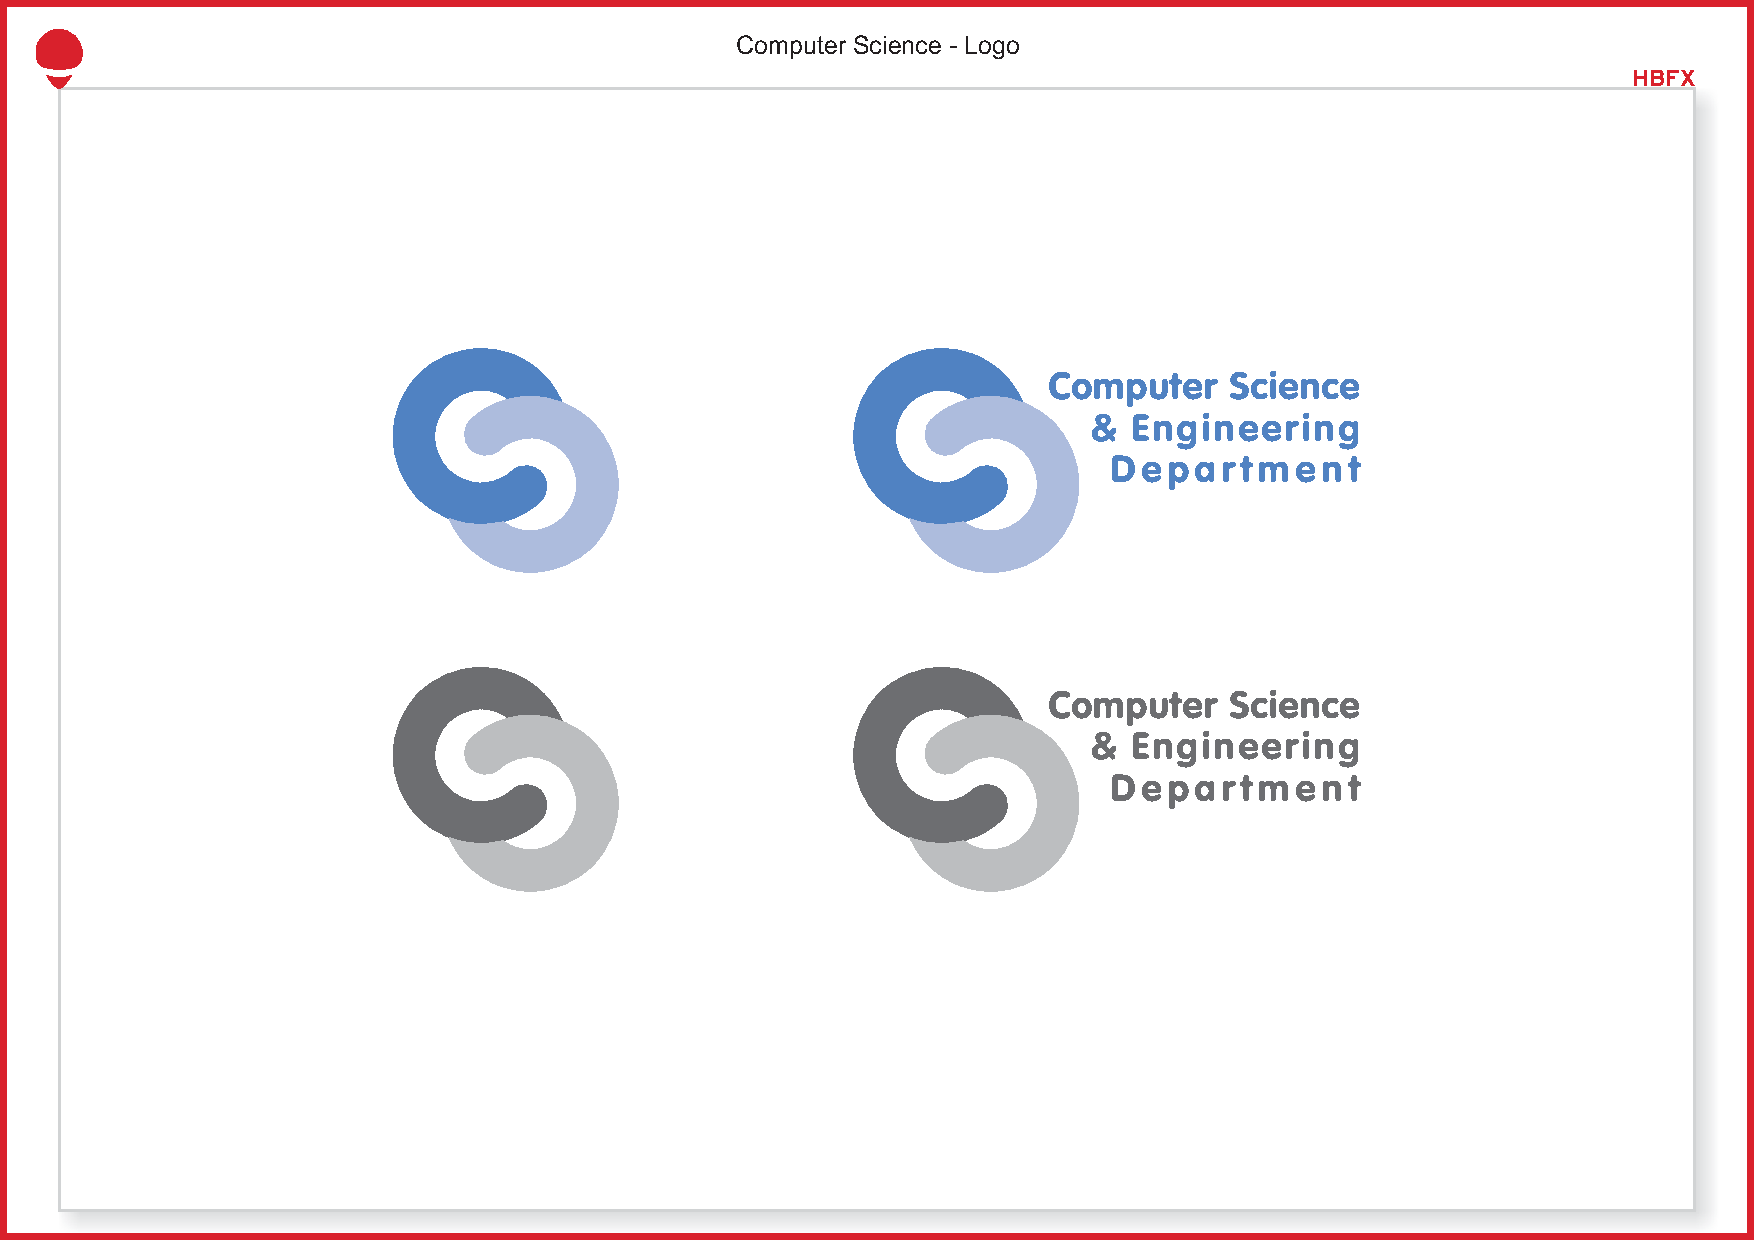
\includegraphics[scale=0.5,trim={14cm 11cm 2cm 5cm},clip=true]{pics/cs-logo.pdf}
\end{tabular}

\vspace{105pt}
{\Huge #2}\\                           % diploma project text
\vspace{40pt}
{\Large #3}\\ \vspace{0pt}  % project title
{\Large #4}\\                          % project subtitle
\vspace{40pt}
{\LARGE \Name}\\                   % student name
\end{center}
\vspace{60pt}
\begin{tabular*}{\textwidth}{@{\extracolsep{\fill}}p{6cm}r}
&{\large\textbf{#5}}\vspace{10pt}\\      % scientific advisor
&{\large \Advisor}                                    % advisor name
\end{tabular*}
\vspace{20pt}
\begin{center}
{\large\textbf{#6}}\\                                % bucharest
\vspace{0pt}
{\normalsize \Year}
\end{center}
\end{titlepage}
}

\newcommand{\frontPageRO}{\frontPage{\UniTextRO}{\DiplomaRO}{\ProjectTitleRO}{\ProjectSubtitleRO}{\AdvisorRO}{\BucRO}}
\newcommand{\frontPageEN}{\frontPage{\UniTextEN}{\DiplomaEN}{\ProjectTitleEN}{\ProjectSubtitleEN}{\AdvisorEN}{\BucEN}}

\linespread{1.5}
\setlength\parindent{0pt}
\setlength\parskip{.28cm}

%% Abstract macro
\newcommand{\AbstractPage}{
\begin{titlepage}
\textbf{\large SINOPSIS}\par
\AbstractRO\par\vfill
\textbf{\large ABSTRACT}\par
\AbstractEN \vfill
\end{titlepage}
}

%% Thank you macro
\newcommand{\ThanksPage}{
\begin{titlepage}
{\noindent \large\textbf{MULȚUMIRI}}\\
\Thanks
\end{titlepage}
}



%%%%%%%%%%%%%%%%%%%%%%%%%%%%%%%%%%%%%%%%%%%%%%%%%%   
%%
%%          End of template definitions
%%   
%%%%%%%%%%%%%%%%%%%%%%%%%%%%%%%%%%%%%%%%%%%%%%%%%%


%%% Puteți elimina aceste linii din lucrare, servesc numai pentru template.
\newcommand{\worktype}[1]{[\textit{#1}] }
\newcommand{\dezvoltare}{\worktype{Dezvoltare de produs}}
\newcommand{\cercetare}{\worktype{Cercetare}}
\newcommand{\ambele}{\worktype{Ambele}}
%%%


%%
%%   Campurile de mai jos trebuie modificate de autor. Modificati doar continutul, nu si numele fiecarei definitii
%%
\newcommand{\ProjectTitleRO}{Yuna, antrenoarea ta virtuală}
\newcommand{\ProjectSubtitleRO}{2018 versiunea 1}
\newcommand{\ProjectTitleEN}{Yuna, your virtual coaching}
\newcommand{\ProjectSubtitleEN}{2018 version 1}
\newcommand{\Name}{Sibel-Leila Bechir}
\newcommand{\Advisor}{Prof. dr. ing. Florica Moldoveanu}
\newcommand{\Year}{2018}

% Setări document
\title{Proiect de diplomă}
\author{\Name}
\date{\Year}

%%
%%   Campurile aferente rezumatului
%%
\newcommand{\AbstractRO}{Sinopsisul proiectului are rol de introducere, conținând atât o descriere pe scurt a problemei abordate cât și o enumerare sumară a rezultatelor și a concluziilor. Se recomandă ca sinopsisul să fie redactat într-un limbaj accesibil unei persoane nefamiliarizate cu domeniul, dar în același timp destul de specific pentru a oferi rapid o vedere de ansamblu asupra proiectului prezentat.
Sinopsisul proiectului va fi redactat atât în română cât și în engleză. Ca dimensiunea recomandată aceasta secțiune va avea maxim 200 de cuvinte pentru fiecare variantă. Împreună, ambele variante se vor încadra într-o singură pagină.}

\newcommand{\AbstractEN}{The abstract has an introductory role and should engulf both a brief description of the issue at hand, as well as an overview of the obtained results and conclusions. The abstract should be formulated such that even somebody that is unfamiliar with the projects’ domain can grasp the objectives of the thesis while, at the same time, retaining a specificity level offering a bird’s eye view of the project.
The projects’ abstract will be elaborated in both Romanian and English. The recommended size for this section is limited to 200 words for each version. Together, both versions will fit in one page.}

%%
%%   Campurile aferente paginii de multumiri
%%
%% \newcommand{\Thanks}{(opțional) Aici puteți introduce o secțiunea specială de mulțumiri / acknowledgments. }

\begin{document}

%%
%%  Prima pagina in romana
%%
\frontPageRO

%%
%%  Prima pagina in engleza
%%
%% \frontPageEN

\begingroup
\linespread{1}
\tableofcontents
\endgroup


% poate fi comentata sau stearsa
%% \ThanksPage

% Textul licentei incepe de aici 
\newpage


%%
%%  Introducere
%%
\chapter{Introducere}

\pagestyle{fancy}

Antrenoarea viruala isi propune sa ajute persoanele aflate in perioada de recaperare a mobilitatii dupa un accident. 

Au existat studii in care s-a demonstrat ca o persoana se poate recupera mai repede in ritmul propriu fata de programul cu constrangeri oferit de centrul specializat de recuperare. 

La centrul de terapie timpul petrecut pe un anumit exercitiu este destul limitat astfel pacientul neputand sa petreaca timpul necesar lui pentru a simti ca il realizeaza corect

% Pacientul poate sa isi extinda timpul necesar pentru realizarea unui exercitiu fata de perioada destul de limitata oferita de programarea la centrul de terapie.

Un alt factor important este rusinea de a pune o intrebari de mai multe ori terapeutului sau persoanei indrumatoarea.

Obiectivul acestui proiect este de a ajuta pacientii aflati in perioada de recuperare prin imbunatatirea progresului prin intermediul unuimediu familiar, precum apartamentul propriu, fata de un mediu necunoscut cum ar fi centrul de recuperare. De asemenea, oferira libertatii de a alege perioada de timp in care se pot face aceste exercitii.

Pentru a se determina cat de bine pacientul exerseaza si cum evolueaza, antrenoarea virtuala, Yuna, va detecta miscarile utilizatorului prin intermediul dispozitivului periferic Kinect. In functie de miscarile utilizatorului, Yuna  va oferi un calificativ acestuia in a il indruma spre a continua exersarea acestui exercitiul sau trecerea la urmatorul nivel de dificulate.


%%
%%  Analiza cerintelor
%%

\chapter{Analiza Cerințelor / Motivație}
\todo[inline, color=red!40]{ Acest capitol va analiza cerințele produsului din prisma potențialilor clienți și a scenariilor de utilizare preconizate, urmând a fi generată o lista de funcționalități. 

Dacă proiectul de licență face parte dintr-un proiect mai amplu (de exemplu un proiect complex, la care lucrează 2 studenți (ex: 1 student la front-end-ul aplicației, 1 student la back-end-ul aplicației), în acest capitol va fi explicat pe scurt ansamblul proiectului și ce parte din proiect este adresată de lucrarea propusă. 

Criterii pentru calificativul \textit{Ne\textit{Satisfăcător}}: 
Cerințele sunt imaginate de student pe baza unei analize a pieței;

Criterii pentru calificativul \textit{Satisfăcător}: 
Există un interviu, un client, analiza cerințelor este elaborată pe baza interviului;

Criterii pentru calificativul \textit{Bine}: 
 Proces iterativ pe baza unor interviuri cu mai mulți clienți, dezvoltare MVP, reevaluare cerințe;
}


%%
%%  Studiu de piata
%%
\chapter{Studiu de Piață}

In momentul actual, exista mai multe aplicatii care prin interediul Kinectului ajuta oamenii sa se recupereze precum si mentinerea formei fizice. Cateva exemple in acest sens sunt:


\section{Recuperarea dupa un atac cerebral}

Cercetatorii din cadrul Microsoft Asia impreuna cu universitatea nationala din Seul au realizat trei aplicatii pentru recuperarea fizica a persoanelor carea au suferit un atac vascular cerebral. 

Acestia au implementat box-and-block test care poate ajuta la evaluarea coordonararii, dexteritatii si capacitatea activității nervoase superioare. Utilizatorii trebuie sa mute cuburi dintr-o parte in alta. Numarul cuburilor mutate va oferi posibilitatea specialistilor de a observa procesul pacientului.

\begin{figure}[th]
\centering
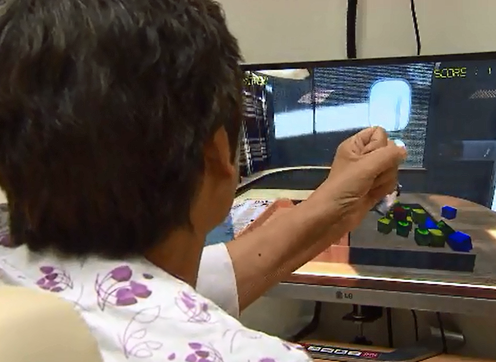
\includegraphics[width=0.6\columnwidth]{modele_existente/Box_and_Block_Stroke_Recovery.png}
  \caption[Box and Block Test]{Box and Block Test\protect\footnotemark}
  \label{figure_1:picture_2}
\end{figure}
\footnotetext{© https://www.microsoft.com/en-us/research/blog/stroke-recovery-gets-a-boost-from-kinect/}

Aceeasi cercetatori au dezvoltat pentru aceasi categorie de persoane o aplicatie in care participantii trebuie sa repete miscarile specialistului filmat. Acest exercitiu este inspirat din Fugl-Meyer Assessment.

Prin intermediul aplicatiei utilizatorul este mult mai relaxat in executarea miscarilor si perioada de recuperare poate reduce semnificativ.

\begin{figure}[th]
\centering
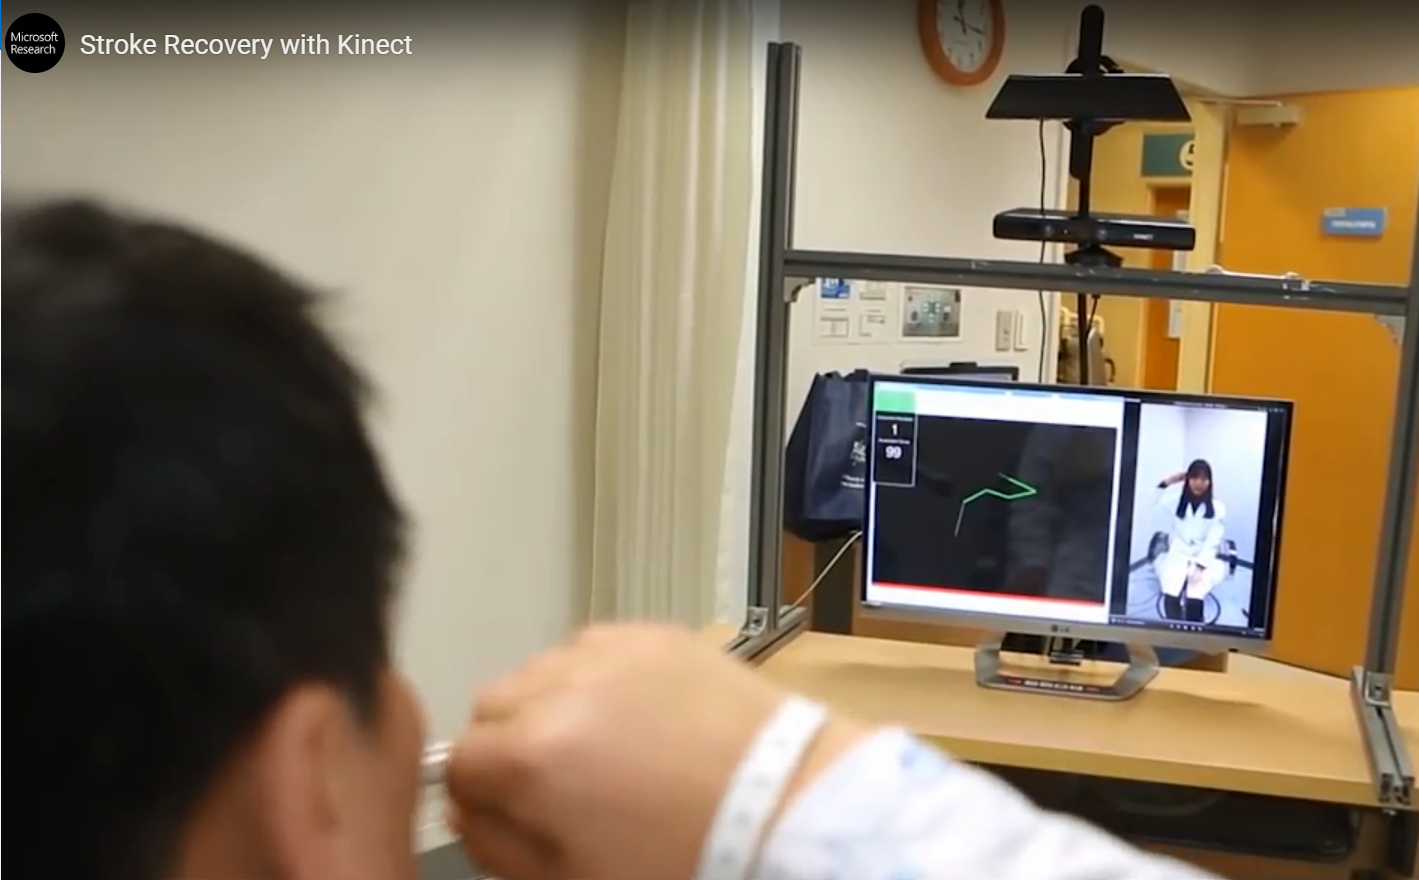
\includegraphics[width=0.6\columnwidth]{modele_existente/Fugl_Meyer_Assessment.png}
  \caption[Fugl-Meyer Assessment]{Fugl-Meyer Assessment\protect\footnotemark}
  \label{figure_1:picture_3}
\end{figure}
\footnotetext{© https://www.microsoft.com/en-us/research/blog/stroke-recovery-gets-a-boost-from-kinect/}

A treia aplicatie este cea in care pacienti isi pot exersa reactia si reflexia. Aceast aspect fiind determinat prin coliziunea dintre racheta condusa de ei si diferiti asteroizi. Miscarile rachetei sunt directionate de pozitia mainii relativ la umar.

\begin{figure}[th]
\centering
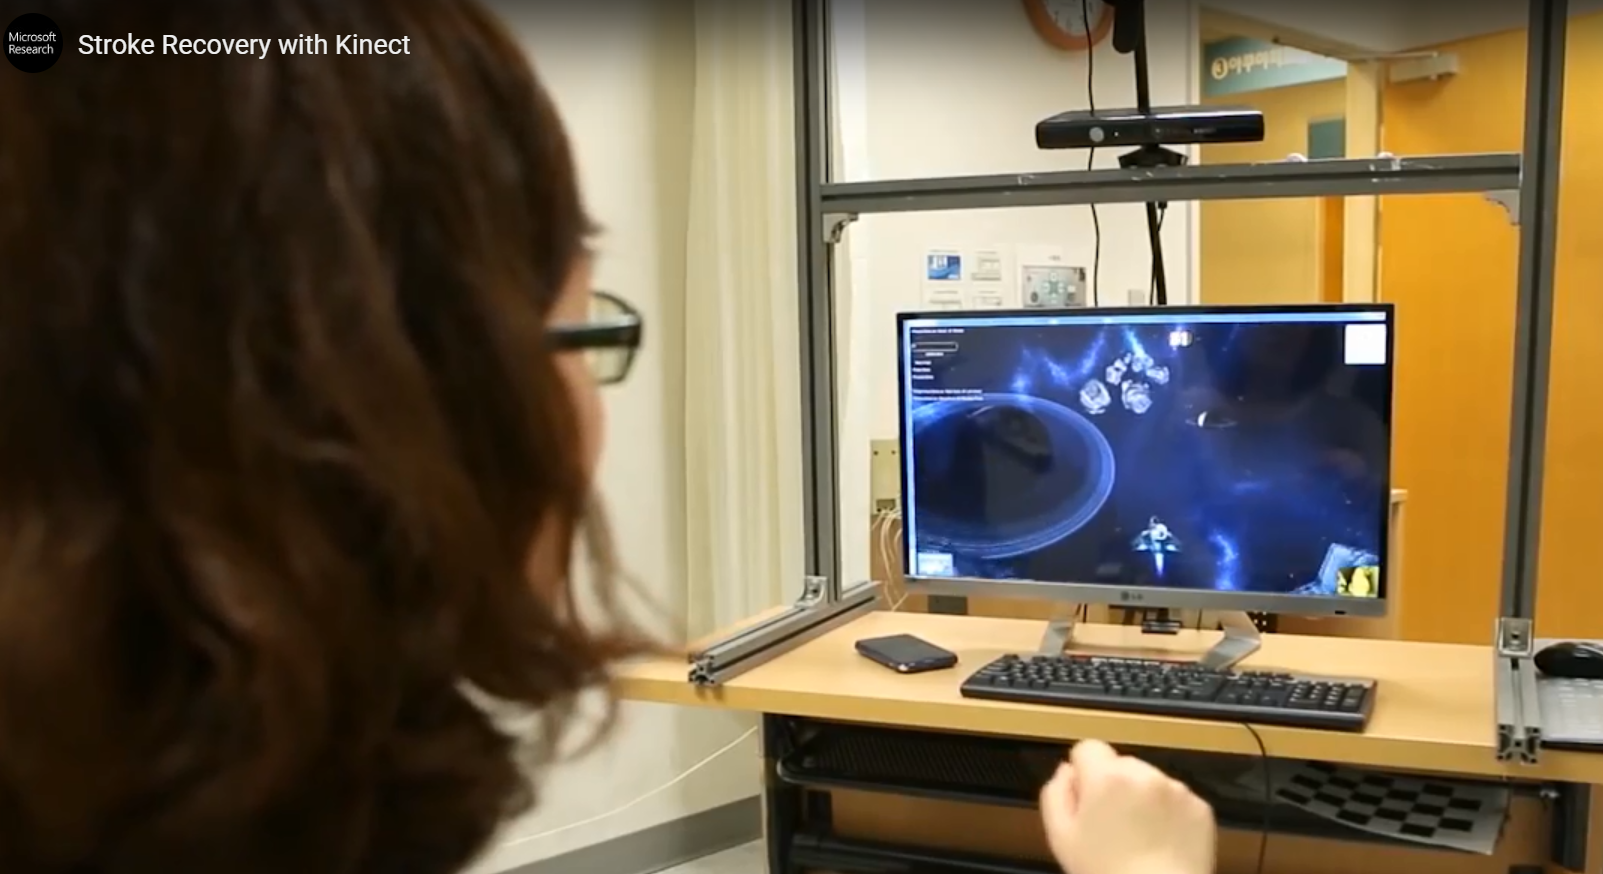
\includegraphics[width=0.6\columnwidth]{modele_existente/outer_space_game.png}
  \caption[Outer space game]{Outer space game\protect\footnotemark}
  \label{figure_1:picture_4}
\end{figure}
\footnotetext{© https://www.microsoft.com/en-us/research/blog/stroke-recovery-gets-a-boost-from-kinect/}

\section{The Biggest Loser: Ultimate Workout}

\textit{The Biggest Loser: Ultimate Workout} este o aplicatie implementa pentru Xbox 360 care cu ajutorul Kinect-ului ajuta utilizatorul sa slabeasca. Aceasta a fost inspirata din serialul televizat \textit{The Biggest Loser}. 

Exercitiile fizice sunt create astfel incat dificulatea sa fie direct proportionala cu evolutia jucatorului precum si particulrizate in functie de varsta si greutea utilizatorului. Contine peste 125 de exercitii si te poti antrene iar un bun element motivational este vocea antrenorilor.

\begin{figure}[th]
\centering
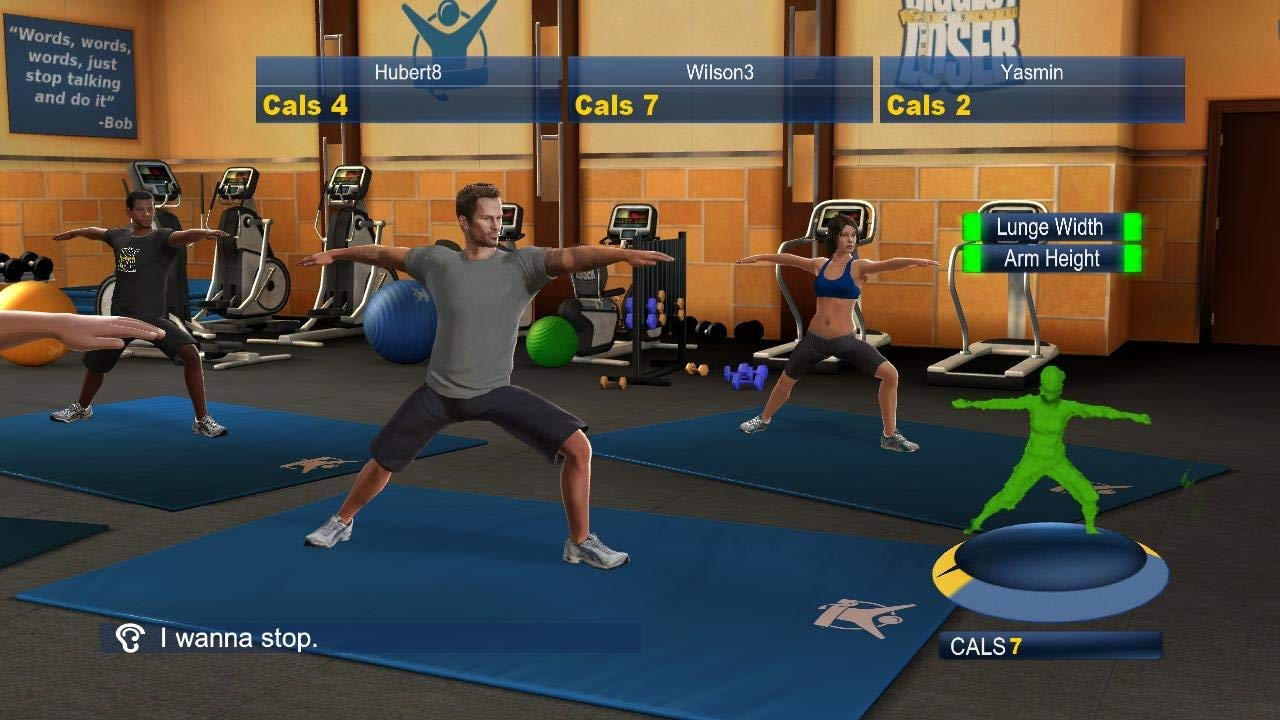
\includegraphics[width=0.6\columnwidth]{modele_existente/The_Biggest_Loser_Ultimate_Workout_Gameplay.jpg}
  \caption[The Biggest Loser Ultimate Workout gameplay]{The Biggest Loser Ultimate Workout gameplay\protect\footnotemark}
  \label{figure_1:picture_5}
\end{figure}
\footnotetext{© https://www.amazon.com/Biggest-Loser-Ultimate-Workout-Xbox-360/dp/B003S2SQFS}

% https://www.google.com/url?sa=i&source=images&cd=&ved=2ahUKEwjHrP_678rgAhUF6KQKHf0oCrsQjRx6BAgBEAU&url=http%3A%2F%2F123kinect.com%2Fkinect-games%2Fthe-biggest-loser-ultimate-workout%2F&psig=AOvVaw3ClV_tzvNqOKaknSJRw9hw&ust=1550771442698655

\section{EA Sports Active 2}

Aceasta aplicatie este dedicata firness-ului si contine 2 device-uri foarte importante care ajuta  in monitorizarea batailor inimii afisate pe ecran. 

Un aspect foarte interesant este dat de contul online al utilizatorului care contine toate antrenamentele, bataiile inimii, numarul de calorii arse precum si alte date importante din istoricul persoanei ceea ce duce la imbunatairea conditiei fizice.

\begin{figure}[th]
\centering
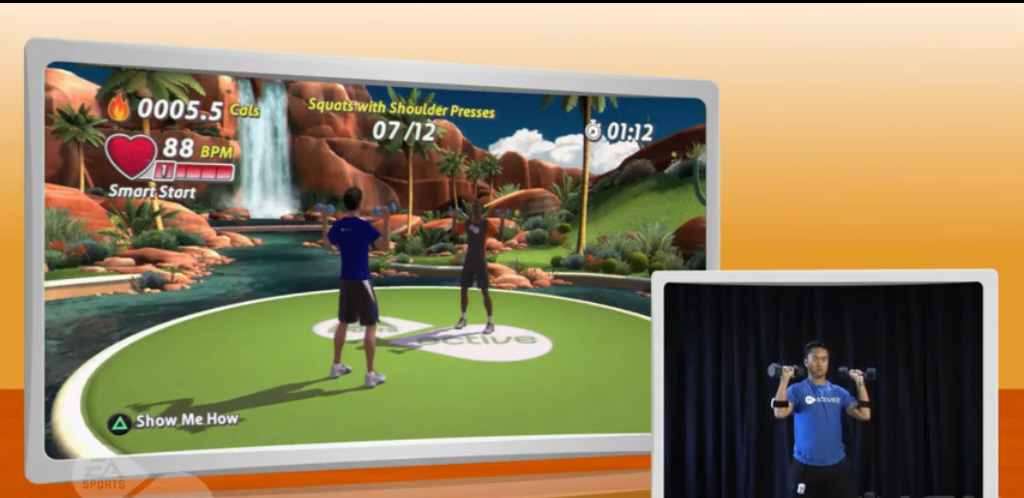
\includegraphics[width=0.7\columnwidth]{modele_existente/EA_Sports_Active_2_gameplay.jpg}
  \caption[EA Sports Active 2 Gameplay]{EA Sports Active 2 gameplay\protect\footnotemark}
  \label{figure_1:picture_6}
\end{figure}
\footnotetext{© https://www.videogamesblogger.com/2010/11/16/ea-sports-active-2-walkthrough-video-guide-xbox-360-ps3-wii.htm}

Prima versiune a fost pe Wii iar in urmatoarea versiune a fost lansata cu ajutorul Microsoft Kinect. In momentul actual EA Sports Active 2 suporta Wii, PlayStation 3 precum si Xbox 360.

%%\begin{figure}[th]
%%\centering
%%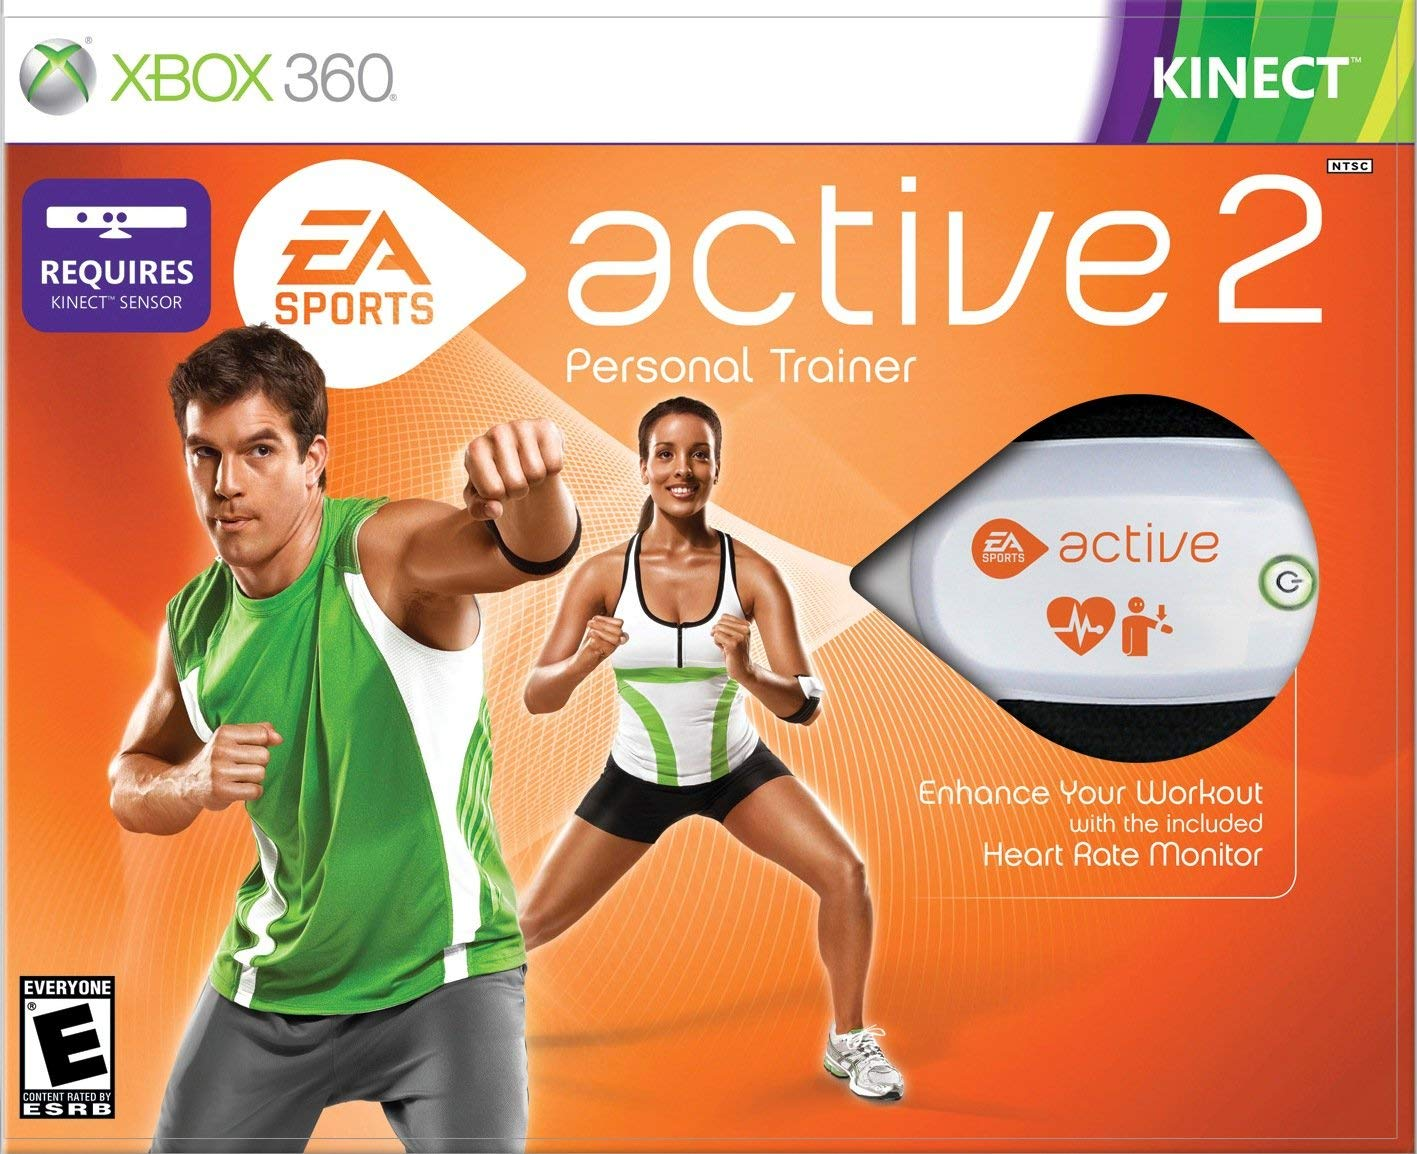
\includegraphics[width=0.4\columnwidth]{modele_existente/EA_Sports_Active_2.jpg}
%%  \caption[EA Sports Active 2]{EA Sports Active 2\protect\footnotemark}
%%  \label{figure_1:picture_7}
%%\end{figure}
%%\footnotetext{© https://images-na.ssl-images-amazon.com/images/}
%%
% https://images-na.ssl-images-amazon.com/images/I/81cgo-6RGzL._AC_SL1417_.jpg

\section{Zumba Fitness Rush - Groove Yourself To Health}

Persoanele care folosesc Zumba Fitness isi mentin forma prin intermediul unor miscari de dans. Aplicatia contine 24 de stiluri internationale de dans oferind un tutorial pentru invatarea fiecarui pas de dans. 

De asemenea, ritmul este foarte alert oferindu-i antrenamentului un nivel ridicat de dificultate si efort. Exercitiile se pot face pe melodiile unor interpreti foarte cunoscuti precum Tiesto, Pitbull precum si alti artisti. 

Zumba Fitness Rush - Groove Yourself To Health a fost dezvoltata de Pipeworks Software si este disponibila pe Wii, PlayStation si Xbox.

\begin{figure}[th]
\centering
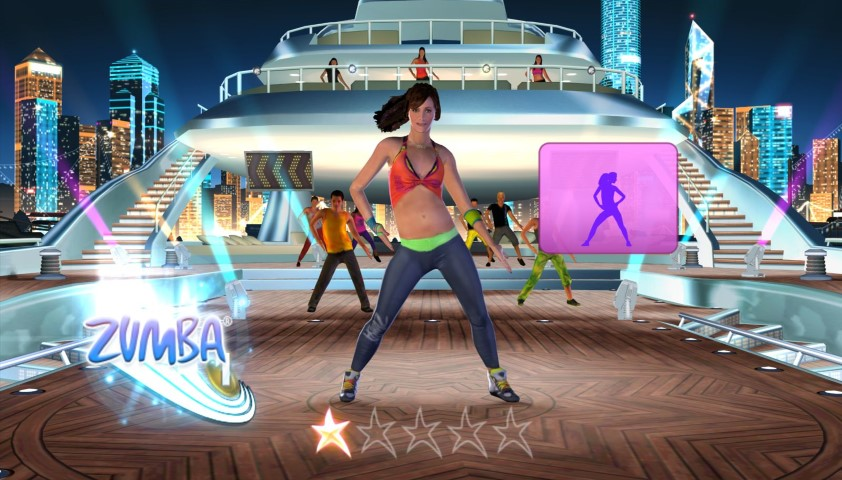
\includegraphics[width=0.6\columnwidth]{modele_existente/Zumba_Fitness.jpg} 
  \caption[Zumba Fitness]{Zumba Fitness\protect\footnotemark}
  \label{figure_1:picture_8}
\end{figure}
\footnotetext{© http://www.impulsegamer.com/360zumbafitnesscore.html}

\section{Shape Up}

Ubisoft a venit cu o un nou nivel pentru antrenamente. Acestea ofera un aspect mai amuzant in executaea miscarilor fizice precum si un timp mai scurt deorece utilizatorii se distreaza.

Un exemplu in acest sent sunt genoflexiunile deoarece cu cat utilizatorul executa mai multe cu atat acesta ajunge mai sus de pe pamant pe spatiu.

Cei din echipa Ubisoft a venit cu ideea de a ilustra obiecte din ce in ce mai mari cu cat se executa mai multe flotari. Acestea pornind de la valize la masini si la elefanti care sunt pozitionati pe spatele utilizatorului.

Aceasta aplicatie a fost creata de Ubisoft numai pentru Xbox One si a fost lansat in noiembrie 2014.

\begin{figure}[th]
\centering
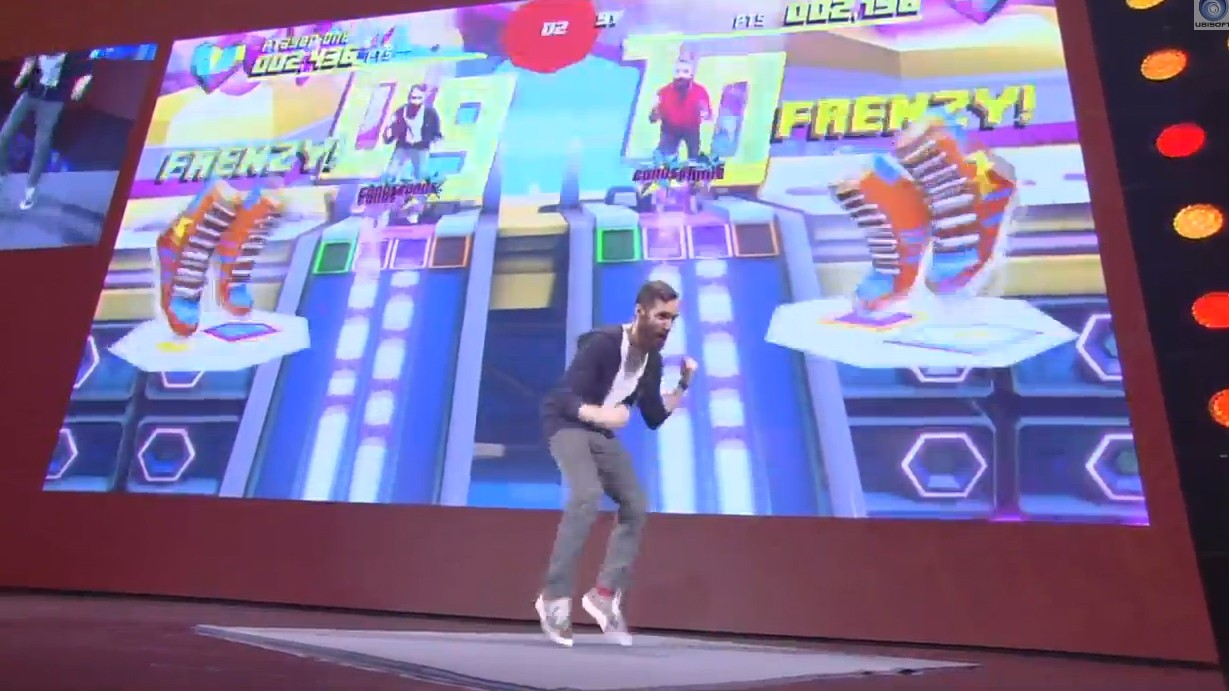
\includegraphics[width=0.6\columnwidth]{modele_existente/Shape_Up.jpg}
  \caption[Shape Up]{Shape Up\protect\footnotemark}
  \label{figure_1:picture_9}
\end{figure}
\footnotetext{© https://www.moddb.com/groups/anime/news/ubisoft-bets-wide}


%%
%%  Detalii de implementare
%%
\chapter{Detalii de implementare}

\section{Crarea avatarului - MakeHuman}

Creatrea caracterului Yunei a fost creat cu ajutorul software-ului open source de creare a humanoizilor tridimensionali, MakeHuman versiunea 1.1.1.

MakeHuman pune la dispozitie un humanoid care poate fi transformat fie in barbat sau femeie. Ca apoi sa il particularizezi mai mult ajutandu-ne de varsta, inaltime, culoarea pielii, forma fetei si forma corpului.

\begin{figure}[th]
\centering
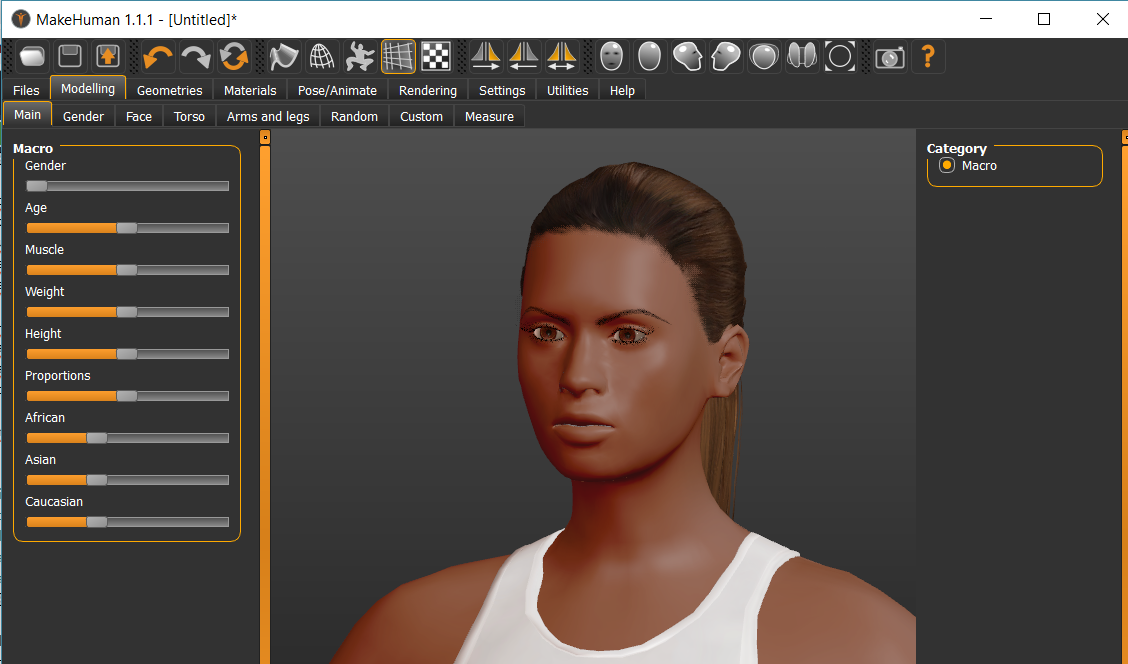
\includegraphics[width=0.6\columnwidth]{modele_existente/MakeHuman_main.png}
  \caption[Customizarea caracterului folosind MakeHuman]{Customizarea caracterului folosind MakeHuman\protect\footnotemark}
  \label{figure_1:picture_11}
\end{figure}

Ajustarea formei corporale este data de proportia intre picioare si abdomen, maini si abdomen, precum si particulatizarea dimensiunii uschiilor pectorali ai spatelui precum si altii. Un aspect interesant este dat de meniul special pentru maini care poate scala dimensiunea manii, lungimea degetelor, lungeamea podului palmei, diametrul degetelor si distanta intre degete.

Am decis ca Yuna sa fie o femeie in varsta de 25 de ani cu o inaltime de 180 de centrimetrii. Alte particularitati speciale adaugate sunt: forma fetei care este ovala, muschii pectorali sunt cu putin mai dezvoltati.

I-am adaugat dinti si limba pentru a oferi mai multa viata caracterului. Acestea sunt vizibile doar atunci cand aceasta mimeaza cuvinte.

MakeHuman ne ofera posibilitatea de a imbraca caracterul la fel si pentru coafura, forma dintilor, forma sprancenelor, lungimea genelelor. Acestea pot sa fie descarcate de pe de pe site-ul comunitatii formate in jurul acestui proiect Open Source http://www.makehumancommunity.org/

Am ales din pachetul default peruca pe care o poarta. Prin intermediul comunitatii online am ales bustiera pantalonii si adidasii acesteia.

Cel mai important lucru care ne ajuta la animatii este ca alegem tipul de rig pe care il vom folosi pentru animatii. Am setat ca ea sa aiba scheletul default astfel fiind o proportie buna intre calitatea animatiilor precum si memoria folosita in crearea acestor animmatii.

\begin{figure}[th]
\centering
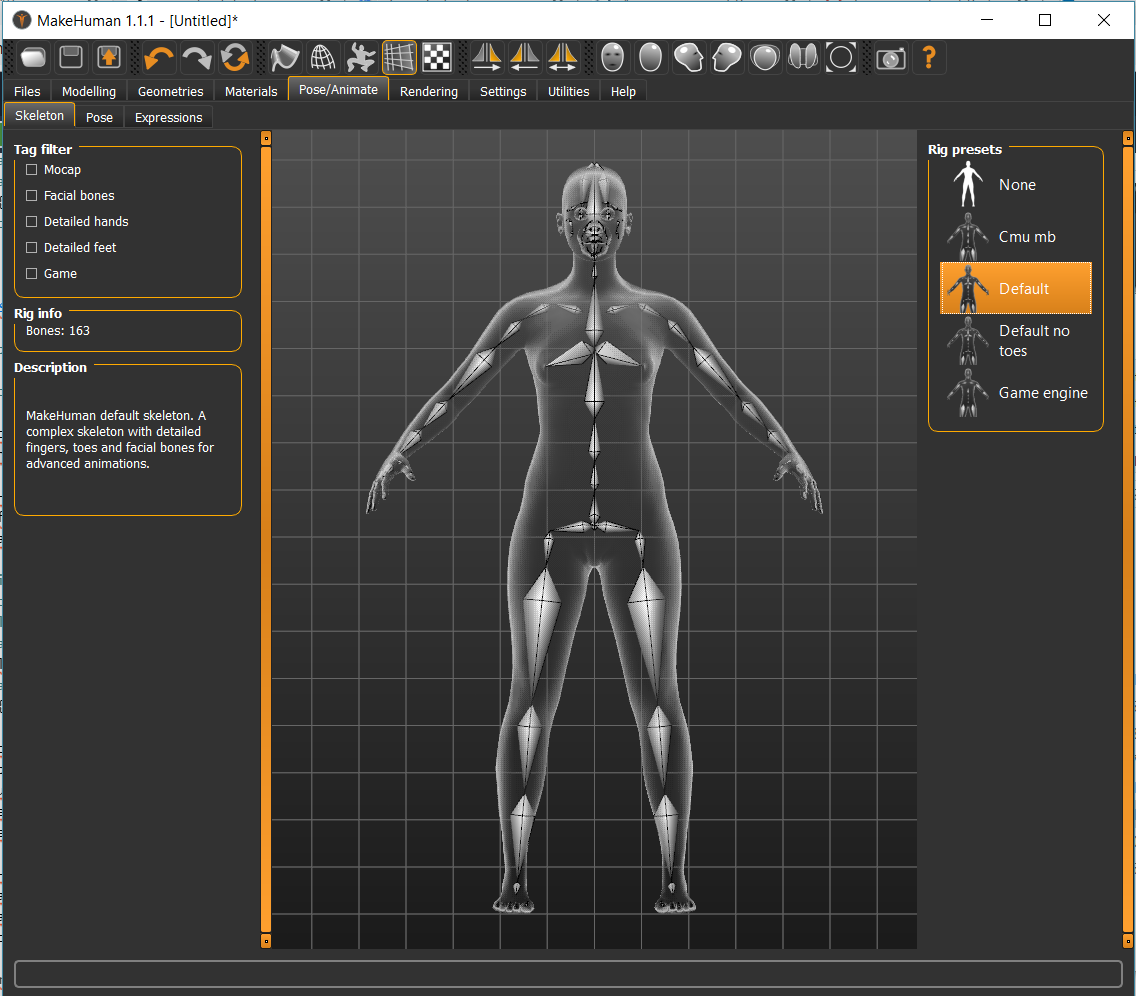
\includegraphics[width=0.45\columnwidth]{modele_existente/MakeHuman_Skeleton.png}
  \caption[Scheletul avatarului]{Scheletul avatarului\protect\footnotemark}
  \label{figure_1:picture_12}
\end{figure}

Un alt aspect tehnic foarte important pe plan tehnic este densitatea mesh-ei de pe caracter.


\begin{figure}[th]
\centering
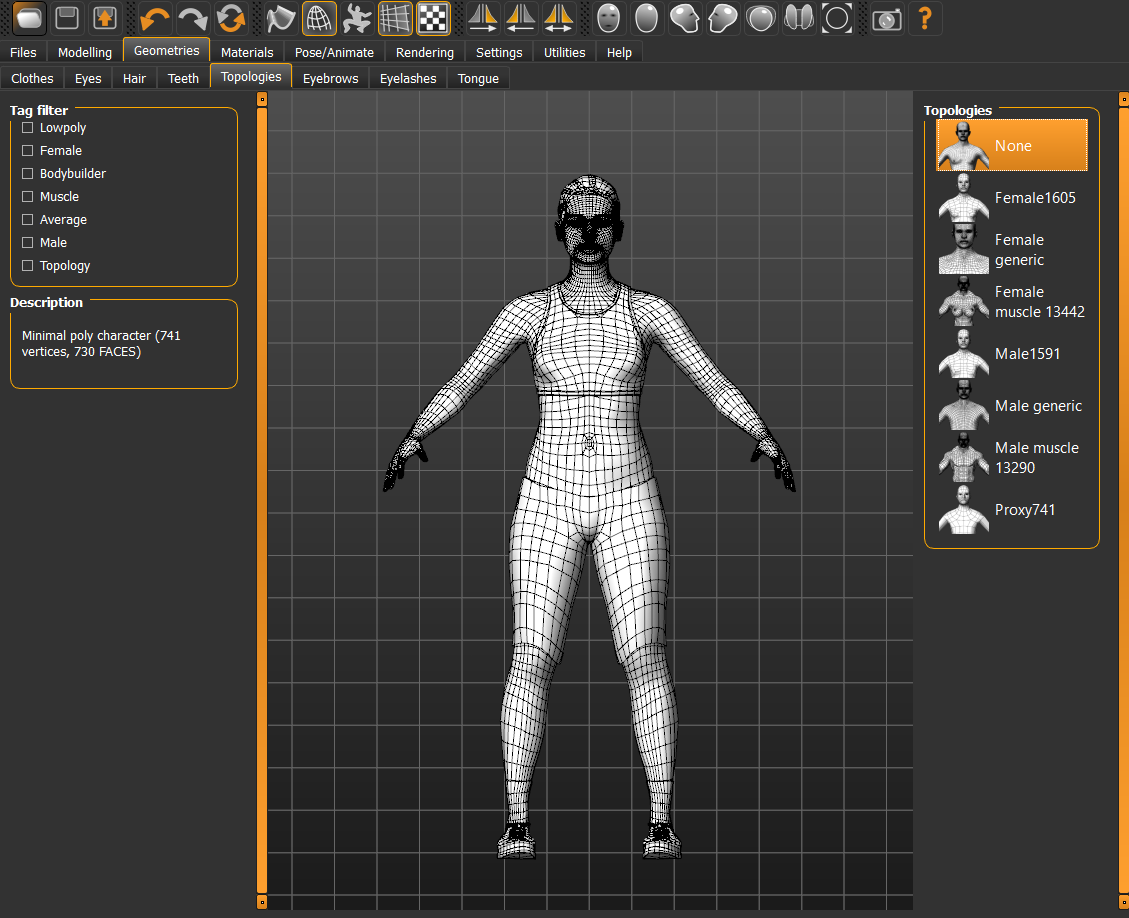
\includegraphics[width=0.45\columnwidth]{modele_existente/MakeHuman_meshDensity.png}
  \caption[Densitatea mesh-ei]{Densitatea mesh-ei\protect\footnotemark}
  \label{figure_1:picture_12}
\end{figure}


\todo[inline, color=blue!40]{}


\section{Schelet}
Dupa cum am vorbit si in sectiunea anterioara, MakeHuman ne ofera posibilitatea de a aduga un schelet 

In cazul Yunei scheletul acesteia este compus din:
\begin{itemize}
    \item sold - coloana - piept - umeri - umar - brat - antebrat - palma - degete
    \item sold - coloana - piept - gat - cap - fata
    \item sold - femur - gamba - picior
\end{itemize}

Sceletul este utilizat pentru a pune restrictii pentru miscarea oaselor.

Pentru ca animatia sa fie implementata pe diferite caractere trebuie sa se foloseasca un schelet omenesc simplist. 


\begin{figure}[th]
\centering
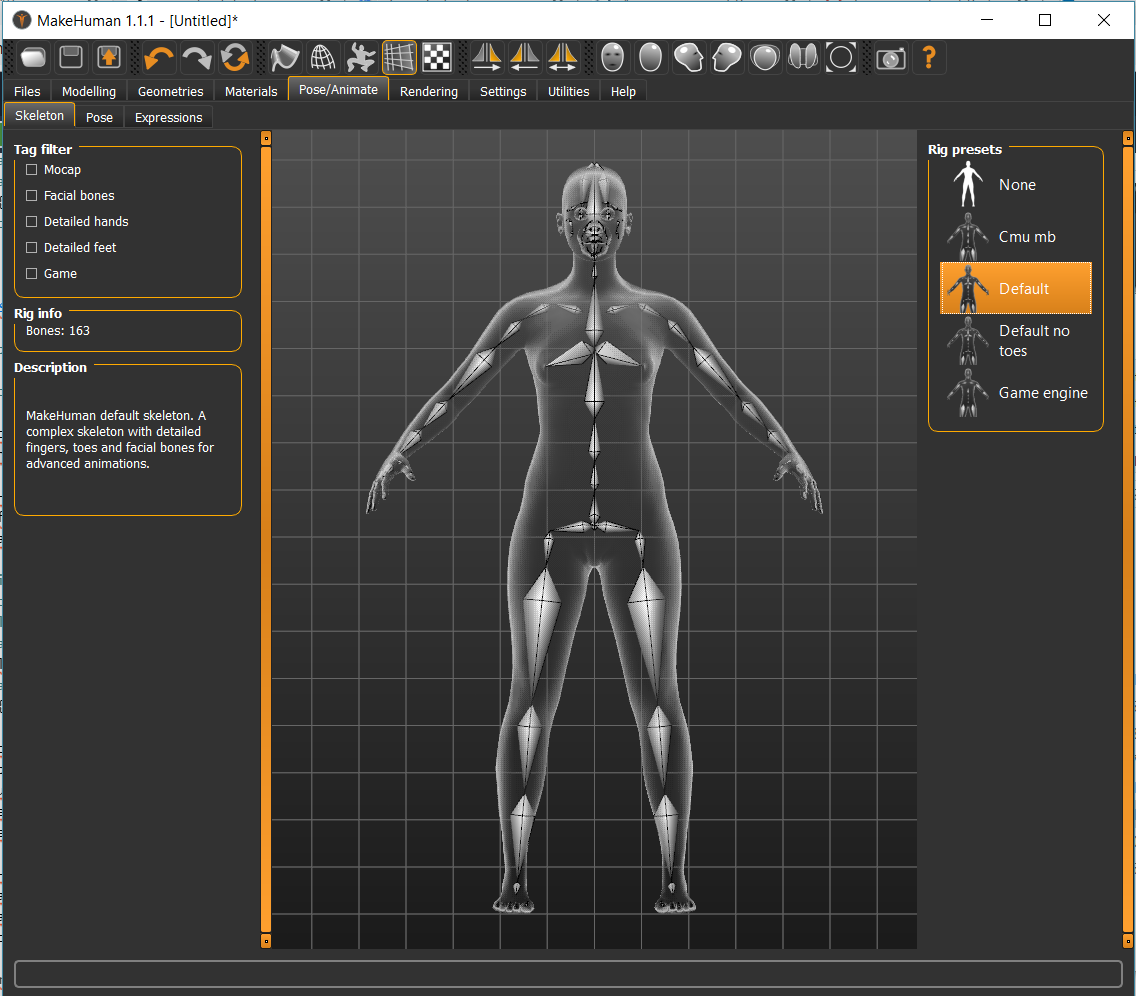
\includegraphics[width=0.45\columnwidth]{modele_existente/MakeHuman_Skeleton.png}
  \caption[Scheletul]{Scheletul\protect\footnotemark}
  \label{figure_1:picture_10}
\end{figure}
\footnotetext{© https://docs.unity3d.com/Manual/UsingHumanoidChars.html}



\section{Animatii - Blender}
Animatiile sunt folosite pentru aducerea la viata a unui obiect prin intermediul miscarilor fiind constituit dintr-o insiruire de frame-uri de-a lungul unei cuante de timp. 

Cel mai important in cadrul unei animatii este humanoidul. Acesta trebuie sa contina obligatoriu:
\begin{itemize}
    \item polygonal mesh
    \item bone structure
    \item skinned for skeleton 
\end{itemize}

Pentru crearea unei animatii se creaza obiectul si il pozitioneaza in key frames care contureaza cele mai importante miscari. Ca pe urma computerul sa genereze cadrele dintre aceste frame-uri.

% https://entertainment.howstuffworks.com/computer-animation1.htm

Pentru a se simula fizica din spatele unui caracter cu aspect uman trebuie ca acesta sa fie format din suprafata caracterului (pielea) si un set de oase interconectate ierarhic (scheletul).


Initial avem datele animatiei in transform space in care putem roti si apoi aceste date se vor translata in spatiul oaselor.

Pentru a crea miscarile unui avatar trebuie sa translatam animation data in ceea ce se numeste spatiul muscular (interiorul corpului).

La baza animatiile pot fi create cu ajutorul:

\begin{itemize}
	\item motion capture (majoritatea fiind create cu ajurorul acesteia)
	\item key frame
	\item biblioteci care pot fi gasite online pe diferite pagini web sau in asseturi
\end{itemize}

Simple datafile stocheaza miscarile caracterului in sceen space precm si in transform space.

Unele animation clips contin caracterul iar altele nu contin caracterul.

Animations clips pot fi 
\begin{itemize}
    \item generice cu extensia FBX
    \item prepraiety din MAX sau Maya
\end{itemize}

Animatiile pot fi create in Unity cu ajutorul ferestrei de animatie. Pentru caractere umane este dificil si nu se recomanda.


\section{blender - Creating animations}
\todo[inline, color=red!40]{https://docs.blender.org/manual/en/latest/animation/index.html}
KeyFrame-urile sunt niste markere in timp care memoreaza coordonatele obiectului.

Animatiile sunt create din keyframe-uri, iar intre cadrele dintre aceste frame-uri sunt interpolari ale keyframe-urilor.

Pentru a oferi iluzia de repetare al miscarilor am memorat la frame-ul end+1 cadrul din primul frame. Dupa ce am terminat animatia i-am dat bake pentru a se memora si frame-urile dintre keyframe-urile principale.

Pentru ca animatiile sa fie 


\section{motion capture}
Crearea animatiilor

Pentru capturarea animatiilor am folosit softwar-ul Ni Mate care este un plugin pentru blender care translateza imaginiile captate de kinect in blender.

Mai multe detalii in link-ul comentat:
% https://www.youtube.com/watch?v=1UPZtS5LVvw&t=327s&fbclid=IwAR3uzhz0WTNn51EMM7O_yH6eD8aiH2hXjTJxPmQoFCYaQKqOVIcHqJG3D3I


%%
%%  Detalii de implementare
%%
\chapter{solutii de pe piata}
\todo[inline, color=red!40]{Ce soluții similare există pe piață? Care sunt limitările lor / pentru ce cazuri de utilizare sau pentru ce tip de clienți produsele existente pe piață nu răspund cerințelor? Care sunt indicatorii pe baza cărora sunt evaluate aceste produse, de către potențiali clienți, și unde sunt lipsurile/ care este oportunitatea generată de lipsurile acestea?}


\ambele În încheierea acestui capitol se dorește descrierea tehnologiilor folosite în lucrare, cu alternative și cu argumente convingătoare calitative și cantitative.  

Criterii pentru calificativul \textit{Ne\textit{Satisfăcător}}: 
\begin{itemize}
	\item \dezvoltare Sunt analizate superficial câteva produse de pe piață; 
	\item \ambele Sunt descrise tehnologiile folosite în lucrare. 
\end{itemize}

Criterii pentru calificativul \textit{Satisfăcător}:
\begin{itemize}
	\item \dezvoltare Există un interviu, un client, analiza cerințelor este elaborată pe baza interviului.
	\item \ambele Sunt descrise câteva tehnologii alternative pentru fiecare din tehnologiile folosite în lucrare. Există o argumentare referitoare la alegere.
\end{itemize}

Criterii pentru calificativul \textit{Bine}:
\begin{itemize}
	\item \dezvoltare Proces iterativ pe baza unor interviuri cu mai mulți clienți, dezvoltare MVP, reevaluare cerințe;
	\item \ambele Sunt descrise tehnologii alternative. Sunt analizate cantitativ și calitativ, folosite benchmarkuri și teste efectuate de student. Analiza este rezumată prin tabele și grafice.
\end{itemize}


%%
%%  Detalii de implementare
%%
\chapter{Soluția Propusă}
\todo[inline, color=red!40]{Capitolul conține o privire de ansamblu a soluției ce rezolvă problema, prin prezentarea structurii / arhitecturii acesteia. În funcție de tipul lucrării acest capitol poate conține diagrame (clase, distribuție, workflow, entitate-relație), demonstrații de corectitudine pentru algoritmii propuși de autor, abordări teoretice (modelare matematică), structura hardware, arhitectura aplicației.}


Criterii pentru calificativul \textit{Ne\textit{Satisfăcător}}: 
\begin{itemize}
	\item	Descriere în limbaj natural.
\end{itemize}

Criterii pentru calificativul \textit{Satisfăcător}: 
\begin{itemize}
	\item	Descriere + diagrame de baze de date, workflow, clase, algoritmi. 
\end{itemize}

Criterii pentru calificativul \textit{Bine}: 
\begin{itemize}
	\item 	Descriere + diagrame de baze de date, workflow, clase, algoritmi + descrierea unui proces prin care s-a realizat arhitectura/structura soluției.
\end{itemize}

\section{Indicații formatare formule}
Formulele matematice utilizate în document vor fi centrate în pagină și numerotate. 

\begin{equation}
(x+a)^n = \sum_{k=0}^{n}\left(\begin{array}{c}n\\k\\\end{array}\right)x^ka^{n-k}
\end{equation}

\begin{equation}
f(x) = a_0 + \sum_{n=1}^{\infty}\left(a_n \cos\frac{n\pi x}{L} + b_n\sin\frac{n\pi x}{L}\right)
\end{equation}


%%
%%  Detalii de implementare
%%
\chapter{Detalii de implementare}
În plus fata de capitolul precedent acesta conține elemente specifice ale rezolvării problemei care au presupus dificultăți deosebite din punct de vedere tehnic. Pot fi incluse configurații, secvențe de cod, pseudo-cod, implementări ale unor algoritmi, analize ale unor date, scripturi de testare. De asemenea, poate fi detaliat modul în care au fost utilizate tehnologiile introduse in capitolul 3.


Criterii pentru calificativul \textit{Ne\textit{Satisfăcător}}: 
\begin{itemize}
	\item	Sunt prezentate pe scurt scheme și pseudo-cod.
\end{itemize}
Criterii pentru calificativul \textit{Satisfăcător}: 
\begin{itemize}
	\item	Descriere sumara a implementării, prezentarea unor secvențe nerelevante de cod, scheme, etc. 
\end{itemize}
Criterii pentru calificativul \textit{Bine}: 
\begin{itemize}
	\item	Descrierea detaliată a algoritmilor/structurilor utilizați; Prezentarea etapizată a dezvoltării, inclusiv cu dificultăți de implementare întâmpinate, soluții descoperite; (dacă este cazul) demonstrarea corectitudinii algoritmilor utilizați. 
\end{itemize}

\section{Indicații formatare tabele}
Se recomandă utilizarea tabelelor de forma celui de mai jos.  Font size :  9. 
Orice tabel prezent în teză va fi referit în text; exemplu: a se vedea Tabel~\ref{tab:criterii}.

\begin{table}[th]\small\linespread{1}
\caption{Sumarizare criterii}
\label{tab:criterii}
\begin{tabular}{l >{\raggedright\arraybackslash}p{8cm} >{\raggedright\arraybackslash}p{4cm}}
\textbf{Calificativ} & \textbf{Criteriu} & \textbf{Observații} \\\hline
\textbf{Nesatisfacator} & Sunt prezentate pe scurt scheme și pseudo-cod & \\\hline
\textbf{Satisfacator} &Descriere sumara a implementării, prezentarea unor secvențe nerelevante de cod, scheme, etc.& \\
\hline
\textbf{\textit{Bine}} &Descrierea detaliată a algoritmilor/structurilor utilizați; Prezentarea etapizată a dezvoltării, inclusiv cu dificultăți de implementare întâmpinate, soluții descoperite; (dacă este cazul) demonstrarea corectitudinii algoritmilor utilizați. & Pot fi incluse configurații, secvente de cod, pseudo-cod, implementări ale unor algoritmi, analize ale unor date, scripturi de testare. \\
\hline
\end{tabular}
\end{table}


\chapter{Evaluare}
Acest capitol trebuie să răspundă, în principiu, la 2 întrebări și să se încheie cu o discuție a rezultatelor obținute. Cele doua întrebări la care trebuie sa se răspundă sunt:
\begin{enumerate}
	\item  \textbf{Merge corect?} (Conform specificațiilor extrase în capitolul 2); 
Evaluarea dacă merge corect se face pe baza cerințelor identificate în capitolele anterioare. 

	\item Cât de \textit{Bine} merge / cum se compară cu soluțiile existente? (pe baza unor metrici clare). 
Evaluarea cât de \textit{Bine} merge trebuie să fie bazată pe procente, timpi, cantitate, numere, \textbf{comparativ cu soluțiile prezentate în capitolul 3}. Poate fi vorba de performanță, overhead, resurse consumate, scalabilitate etc. 
\end{enumerate}

În realizarea discuției, se vor utiliza tabele cu procente, rezultate numerice și grafice. În mod obișnuit, aici se fac comparații și teste comparative cu alte proiecte similare (dacă există) și se extrag puncte tari și puncte slabe. Se ține cont de avantajele menționate și se demonstrează viabilitatea abordării / aplicației, de dorit prin comparație cu alte abordări (dacă acest lucru este posibil). Cuvântul cheie la evaluare este ``metrică'': trebuie să aveți noțiuni măsurabile și cuantificabile. În cadrul procesului de evaluare, explicați datele, tabelele și graficele pe care le prezentați și insistați pe relevanța lor, în următorul stil: ``este de preferat ... deoarece …''; explicați cititorului nu doar datele ci și semnificația lor și cum sunt acestea interpretate. Din această interpretare trebuie să rezulte poziționarea proiectului vostru printre alternativele existente, precum și cum poate fi acesta îmbunătățit în continuare.

Criterii pentru calificativul \textit{Ne\textit{Satisfăcător}}: 
\begin{itemize}
	\item Aplicația este testată dar rulează pe calculatorul studentului, nu există posibilități de testare, nu a fost validată cu clienți / utilizatori;
	\item Nu au fost realizate comparații cu alte sisteme similare.
\end{itemize}

Criterii pentru calificativul \textit{Satisfăcător}: 
\begin{itemize}
	\item \dezvoltare  Există teste unitare și de integrare, există o strategie de punere în funcțiune (deployment), există validare minimală cu clienții / utilizatorii.
	\item \ambele Discuție minimală asupra relevanței rezultatelor prezentate, comparație minimală cu alte sisteme similare.
\end{itemize}

Criterii pentru calificativul \textit{Bine}: 
\begin{itemize}
	\item \dezvoltare Teste unitare și de integrare, instrumente de punere in funcțiune (deployment) utilizate și care arată lucru constant de-a lungul semestrului, lucrare validată cu clienții / utilizatorii, produs în producție.
	\item \ambele Discuție cu prezentarea calitativă și cantitativă a rezultatelor, precum și a relevanței acestor rezultate printr-o comparație complexă cu alte sisteme similare.
\end{itemize}

\chapter{Concluzii}
În acest capitol este sumarizat întreg proiectul, de la obiective, la implementare, si la relevanta rezultatelor obținute. În finalul capitolului poate exista o subsecțiune de ``Dezvoltări ulterioare''.

Criterii pentru calificativul \textit{Ne\textit{Satisfăcător}}: 
\begin{itemize}
	\item	Concluziile nu sunt corelate cu conținutul lucrării;
\end{itemize}

Criterii pentru calificativul \textit{Satisfăcător}: 
\begin{itemize}
	\item	Concluziile sunt corelate cu conținutul lucrării, însă nu se oferă o imagine asupra calității și relevantei rezultatelor obținute;
\end{itemize}

Criterii pentru calificativul \textit{Bine}: 
\begin{itemize}
	\item	Concluziile sunt corelate cu conținutul lucrării, și se oferă o imagine precisa asupra relevantei și calității rezultatelor obținute în cadrul proiectului. 
\end{itemize}


%%
%%  Detalii de implementare
%%
\chapter*{Bibliografie}\addcontentsline{toc}{chapter}{Bibliografie}  
% * <marios.choudary@gmail.com> 2018-02-28T12:07:48.730Z:
% 
% > BIBLIOGRAFIE
% Am adaugat un paragraf cu cateva detalii despre folosirea citarilor bibliografice in Latex, despre folosirea lui "\cite" si despre posibilitatea folosirii bibliografiei si direct in fisierul Latex.
% 
% ^.

\begin{itemize}
	\item 	NU utilizați referințe la Wikipedia sau alte surse fără autor asumat.
	\item 	Pentru referințe la articole relevante accesibile în web (descrise prin URL) se va nota la bibliografie și data accesării.
	\item 	Mai multe detalii despre citarea referințelor din internet se pot regăsi la:
	\begin{itemize}
		\item	\url{http://www.writinghelp-central.com/apa-citation-internet.html}
		\item	\url{http://www.webliminal.com/search/search-web13.html}
	\end{itemize}
	\item 	Note de subsol se utilizează dacă referiți un link mai puțin semnificativ o singură dată; Dacă nota este citată de mai multe ori, atunci utilizați o referință bibliografică.
	\item 	Dacă o imagine este introdusă în text și nu este realizată de către autorul lucrării, trebuie citată sursa ei (ca notă de subsol sau referință - este de preferat utilizarea unei note de subsol).
	\item 	Referințele se pun direct legate de text (de exemplu ``KVM [1] uses'', ``as stated by Popescu and Ionescu [12]'', etc.). Nu este recomandat să folosiți formulări de tipul ``[1] uses'', ``as stated in [12]'', ``as described in [11]'' etc..
	\item 	Afirmațiile de forma ``are numerous'', ``have grown exponentially'', ``are among the most used'', ``are an important topic'' trebuie să fie acoperite cu citări, date concrete si analize comparative.
	\begin{itemize}
		\item	Mai ales în capitolele de introducere, ``state of the art'', ``related work'' sau ``background'' trebuie să vă argumentați afirmațiile prin citări. Fiți autocritici și gândiți-vă dacă afirmațiile au nevoie de citări, chiar și cele pe care le considerați evidente.
		\item	Cea mai mare parte dintre citări vor fi în capitolele de introducere ``state of the art'', ``related work'' sau ``background''.
	\end{itemize}
	\item 	Toate intrările bibliografice trebuie citate în text. Nu le adăugați pur și simplu la final.
	\item 	Nu copiați sau traduceți niciodată din surse de informație de orice tip (online, offline, cărți, etc.). Dacă totuși doriți să oferiți, prin excepție, un citat celebru - de maxim 1 frază- utilizați ghilimele și evident menționați sursa. .
	\item 	Dacă reformulați idei sau creați un paragraf rezumat al unor idei folosind cuvintele voastre, precizați cu citare (referință bibliografică) sau cu notă de subsol sursa sau sursele de unde ați preluat ideile.
\end{itemize}

Trebuie respectat un singur standard de trimiteri bibliografice (citare), dintre următoarele alternative:
\begin{itemize}
	\item APA (\url{http://pitt.libguides.com/c.php?g=12108\&p=64730})
	\item IEEE (\url{https://ieee-dataport.org/sites/default/files/analysis/27/IEEE\%20Citation\%20Guidelines.pdf}) 
	\item Harvard (\url{https://libweb.anglia.ac.uk/referencing/harvard.htm})
	\item Cu numerotarea referințelor în ordine alfabetică sau în ordinea apariției în text (de exemplu, stilul cu numere folosit de unele publicații ACM - \url{https://www.acm.org/publications/authors/reference-formatting}) 
\end{itemize}

În Latex este foarte ușor să folosiți referințe într-un mod corect și unitar, fie prin adăugarea unei secțiuni
\verb!\begin{thebibliography}!
(vezi la sfârșitul acestei secțiuni), fie printr-un fișier separat de tip bib, folosind comanda
\verb!\bibliography{}!,
așa cum procedăm mai jos prin folosirea fișierului ``bibliography.bib''. În orice caz, în Latex va trebui să folosiți comanda
\verb!\cite{}!
pentru a adăuga referințe, iar această comandă trebuie folosită direct în text, acolo unde vreți sa apară citația, ca în exemplele următoare:
\begin{itemize}
	\item Articol jurnal: ~\cite{article};
	\item Articol conferință:~\cite{proc};
	\item Carte: ~\cite{book};
	\item Weblink: ~\cite{silva};
\end{itemize}

\textbf{Important}: în această secțiune de obicei apar doar intrările bibliografice (adică doar listarea referințelor). Citarea lor prin comanda cite și explicații legate de ele trebuie facute în secțiunile anterioare. Citarea de mai sus a fost facută aici doar pentru exemplificare.

% Asa se specifica folosirea unui fisier cu referinte bibliografice:
\bibliographystyle{plain}
\bibliography{bibliography}

%% O alta varianta ar fi fost includerea de articole direct in acest fisier
%% in felul urmator:
%% \begin{thebibliography}{ABC}
%%
%% \bibitem{article}
%%  H. Baali, H. Djelouat, A. Amira and F. Bensaali,
%%  ``Empowering Technology Enabled Care Using IoT and Smart Devices:
%   A Review''. In: IEEE Sensors Journal, vol. 322 (10), pp. 891--921, 1905.
%%
%% (more \bibitem items here...)
%%
%% \end{thebibliography}

%% Daca vreti ca o sectiune sa inceapa pe o pagina noua, puteti forta acest lucru cu comanda "\newpage", ca mai jos:

%\newpage

\chapter*{Anexe}\addcontentsline{toc}{chapter}{Anexe}

Anexele sunt opționale.
Ce poate intra în anexe:
\begin{itemize}
\item	Exemplu de fișier de configurare sau compilare;
\item	Un tabel mai mare de o jumătate pagină;
\item	O figura mai mare mai mare de jumătate pagină;
\item	O secvență de cod sursa mai mare de jumătate pagină;
\item	Un set de capturi de ecran (``screenshot''-uri);
\item	Un exemplu de rulare a unor comenzi plus rezultatul (``output''-ul) acestora;
\item 	În anexe intră lucruri care ocupă mai mult de o pagină ce ar întrerupe firul natural de parcurgere al textului.
\end{itemize}

\begin{appendices}

\chapter{Extrase de cod} % Introduce o nouă anexă
\ldots


\end{appendices}
\end{document}